%
% appendix.tex
%
% Copyright (C) 2015, Achim Lösch <achim.loesch@upb.de>, Christoph Knorr <cknorr@mail.uni-paderborn.de>
% All rights reserved.
%
% This documentation may be modified and distributed under the terms
% of the BSD license. See the LICENSE file for details.
%
% encoding: UTF-8
% tab size: 4
%
% author: Christoph Knorr (cknorrh@mail.uni-paderborn.de)
% created: 7/27/14
% version: 0.5.8 - change project name to ampehre
%          0.6.0 - add ioctl for the ipmi timeout, new parameters to skip certain measurements 
%                  and to select between the full or light library. 
%

\section{Recommended Sampling Rates} \label{app:A}
Users must specify a sampling rate for each resource which is compiled as libmeasure module. The sampling rate defines how often measurement values are queried from the devices. Low sampling rates can produce substantial CPU load, since all the measurement threads are executed on the CPU. Hence, sampling rates have to be chosen carefully. Moreover, they have an impact on the accuracy of the measurement results and the CPU utilization. We have to find a trade-off between accuracy of the measurements and the CPU utilization which also leads to different CPU power consumption. Therefore we have methodically examined different sampling rate combinations using all five modules runnable on our heterogeneous system. We have used libmeasure in its \texttt{VARIANT\_FULL} (all sensors are sampled) with high accuracy (\texttt{skip\_ms\_rate} set to \texttt{SKIP\_NEVER}). We have measured the power consumption and utilization while all resources have been in idle state. The results are shown in Figure \ref{fig:CPUUtilization} and \ref{fig:CPUPower}. Obviously, the CPU utilization and power consumption is highly dependent on specific system configurations. We hope that our results are helpful anyway.\\

Figure \ref{fig:CPUUtilization} shows the CPU utilization, sampling all sensors of all currently supported resources as specified in Section \ref{sec:hardware}. The lines indicate our recommendations to achieve utilizations below a specific thresholds. For example, the blue line indicates that the utilization induced by our measuring library loading all resource-specifc modules stays below 2 \%, if the sampling rates CPU: 40 ms, MIC: 50 ms, GPU: 40 ms, FPGA: 70 ms and System 100 ms or higher are used for the measurements.

\begin{figure}[!h]
\begin{center}
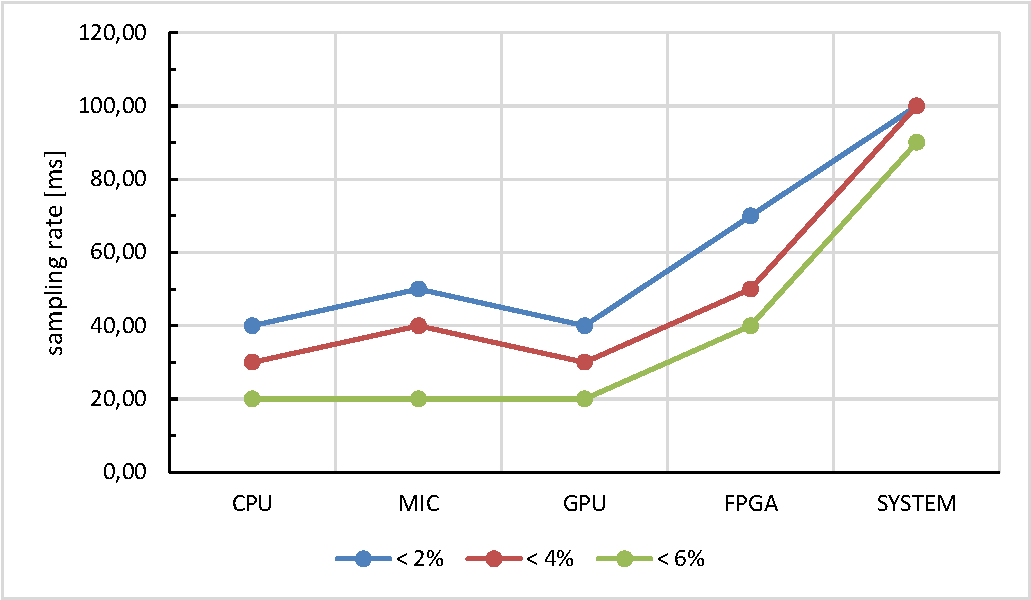
\includegraphics[width=\textwidth]{CPUUtilization} 
\caption{Libmeasure sampling rates and the resulting CPU utilization in percent. The lines indicate the lower boundaries of the sampling rates for which the CPU utilization is not higher than the corresponding threshold (2 \%, 4 \%, 6 \%).}
\label{fig:CPUUtilization}
\end{center}
\end{figure}

Figure \ref{fig:CPUPower} shows the resulting CPU power consumption induced by sampling all sensors of all currently supported resources as specified in Section \ref{sec:hardware}. Accordingly, the lines indicate what sampling rates have to be chosen to make sure that the CPU power consumption stays below specific thresholds. For example the sampling rates have to be CPU: 20 ms, MIC: 20 ms, GPU 30 ms, FPGA 40 ms, System 80 ms or higher to get a CPU power consumption of less than 18 W.\\

\begin{figure}[!h]
\begin{center}
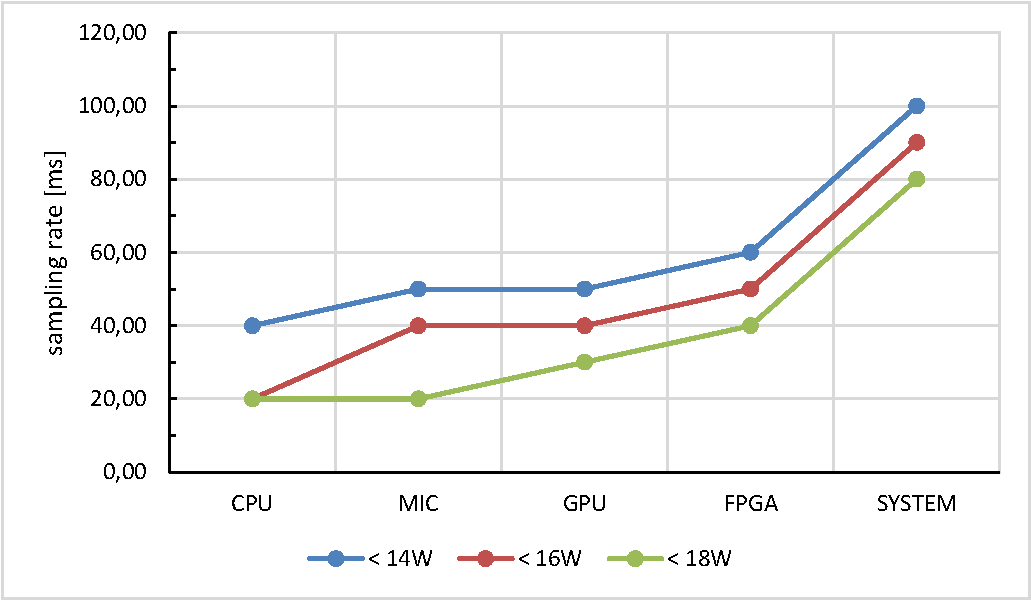
\includegraphics[width=\textwidth]{CPUPower} 
\caption{Libmeasure sampling rates and the resulting CPU Power consumption in Watt. The lines indicate the lower boundaries for which the CPU power consumption is not higher than the corresponding threshold (14 W, 16 W, 18 W).}
\label{fig:CPUPower}
\end{center}
\end{figure}

